\documentclass{exam}

\usepackage{units} 
\usepackage{xfrac} 
\usepackage[fleqn]{amsmath}
\usepackage{cancel}
\usepackage{float}
\usepackage{mdwlist}
\usepackage{booktabs}
\usepackage{cancel}
\usepackage{polynom}
\usepackage{caption}
\usepackage{fullpage}
\usepackage{comment}
\usepackage{enumerate}
\usepackage{graphicx}

\newcommand{\degree}{\ensuremath{^\circ}} 
\everymath{\displaystyle}

\printanswers

\ifprintanswers 
  \usepackage{2in1, lscape} 
\fi

\author{}
\date{January 29, 2014}
\title{Statistics \\ Homework One}

\begin{document}

  \maketitle

  \ifprintanswers
  \else
    \begin{itemize*}
      \item read Chapter 2 
      \item answer the questions in ``Check Your Skills'' and check the answers in the back of the book
      \item hand in exercises TO DO
    \end{itemize*}
  \fi

  \ifprintanswers
    \begin{description}
      \item[25] The larger number is the mean because the mean is dragged upward by a few people who make hundreds of
        thousands of dollars.

      \item[26] For the people who are still working (21-64), there are a lot of young people with almost no retirement
        money and a few older people with large retirement accounts.  This makes the distribution right-skewed and the
        mean is larger than the median.

        For the people who are mostly retired (55 or older), almost everyone has some retirement money saved, and there
        are only a few people with no retirement money.  This makes the distribution left-skewed and the mean is smaller
        than the median.

      \item[27] 
        \begin{itemize*}
          \item the median is college 393
          \item the first quartile is college 197
          \item the third quartile is college 590
        \end{itemize*}

      \item[29]
        \begin{figure}[H]
          \centering
          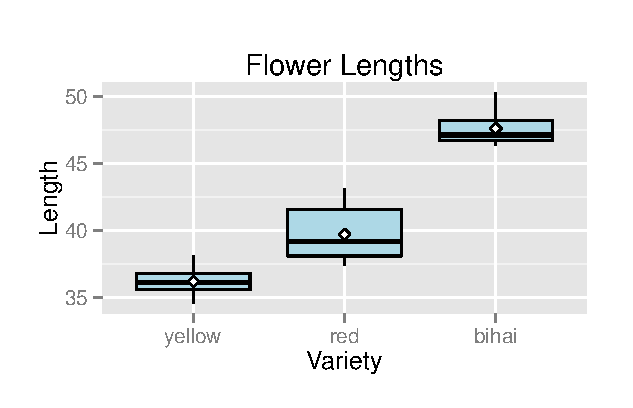
\includegraphics{figures/ex29.eps}
          \caption{Exercise 29}
        \end{figure}

        \begin{table}[ht]
          \centering
          \begin{tabular}{rlrrrrrr}
            \toprule
              & Variety & Min.  & 1st Qu. & Median & Mean  & 3rd Qu. & Max. \\
            \midrule
            1 & bihai   & 46.34 & 46.73   & 47.12  & 47.60 & 48.20   & 50.26 \\
            2 & red     & 37.40 & 38.08   & 39.16  & 39.71 & 41.58   & 43.09 \\
            3 & yellow  & 34.57 & 35.56   & 36.11  & 36.18 & 36.80   & 38.13 \\
            \bottomrule
          \end{tabular}
        \end{table}

        The summary doesn't show the shape that the histogram does.

      \item[30]
        If you add up all the bars, you find that there are 78 girls.  The median would be between girl number 39 and
        40, which would be in the 2 servings bar.  The first quartile would be girl 19 which is in the 1 serving bar and
        the third quartile would be girl 59 which is in the 4 servings bar.  So the answer is:

        \begin{itemize*}
          \item first quartile: 1
          \item median: 2
          \item third quartile: 4
        \end{itemize*}
        
      \item[32]
        \begin{parts}
          \part symmetric distributions without outliers

          \part 
            \begin{itemize*}
              \item for the men, $\bar{x}$ went from 117.17 to 110.86 and $s$ went from 74.24 to 66.88
              \item for the women, $\bar{x}$ went from 165.17 to 158.45 and $s$ went from 56.51 to 43.65
            \end{itemize*}

        \end{parts}

      \item[37]
        The average of the individual state averages is only 8.5\%.

        The big states have more people so they have a greater affect on the national average than the small states.
        Since the big states all have high percentages of foreign-born people, the national average is higher than the
        average of all the states individually.

      \item[38]
        For the median to be zero, half the households must have no credit card debt.  There are probably quite a few
        households that have not credit cards at all, so they don't have any credit card debt.  And even if you just
        look at credit card holders, there are probably quite a few people who pay their credit cards every month and
        don't have any debt.


      \item[39]
        \begin{parts}
          \part You can get a standard deviation of 0 by choosing the same number four times.

          \part You get the maximum standard deviation by choosing two 0s and two 10s.

          \part Any number works for part a.  There is only one correct answer for part b.
        \end{parts}

      \item[41]
        For the mean to be 7, the five numbers must add up to 35.  For the median to be 10, the third number in the
        sequence must be 10.

        Since the mean needs to be less than the median, it makes sense to use as small numbers as possible.  If the
        last three numbers are all 10s, the middle number will be 10.  Then the first two numbers need to add to 5 to
        get the total to 35.

        A few sets of numbers that work with this approach are: 
        
        \{1, 4, 10, 10, 10 \} and \{2, 3, 10, 10, 10\}.

        Once you see this, you can make other choices for the last two numbers, as long as you don't make them so large
        that you can't get the mean down to 7.  

      \item[42]
        For the mean to be larger than the third quartile, you just need one really large number.  Here is a set that
        works: 
        
        \{1, 2, 3, 4, 5, 100 \}.  
        
        The third quartile is 5 and the mean is 19.17.

      \item[43]
        \begin{table}[ht]
          \centering
          \begin{tabular}{rr}
            \toprule
            Min.    & 380,000 \\
            1st Qu. & 425,000 \\
            Median  & 2,800,000 \\
            Mean    & 5,066,000 \\
            3rd Qu. & 8,250,000 \\
            Max.    & 17,020,000 \\
            \bottomrule
          \end{tabular}
          \caption{Summary}
        \end{table}

        \begin{figure}[H]
          \centering
          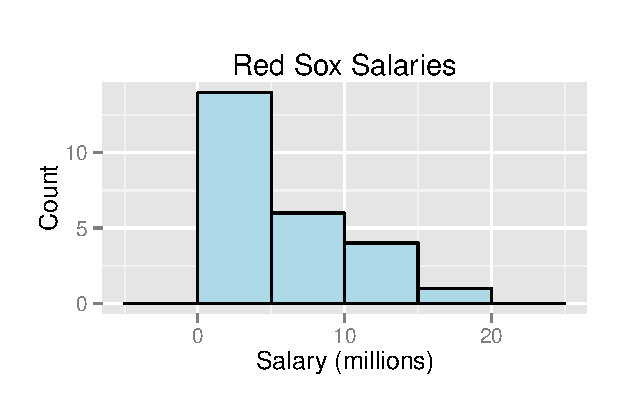
\includegraphics{figures/ex43.eps}
          \caption{Exercise 43 Histogram}
        \end{figure}

        The summary for the owner might be:
        \begin{itemize*}
          \item half the players make \$2.8M or less
          \item Manny Ramirez is the highest paid player on the team at \$1.7M.  Curt Schilling and David Ortiz are next
            at \$1.3M.
          \item The top three players (Ramirez, Schilling, and Ortiz) account for 35\% of the payroll
          \item Jacoby Ellsbury, Manny Delcarmen and Dustin Pedroia are the lowest paid players at \$380,000.
          \item The mean salary is \$5M.
          \item The total payroll is \$127M
        \end{itemize*}

      \item[44]
        \begin{table}[H]
          \centering
          \begin{tabular}{rlrr}
            \toprule
              & Odor     & Median & Mean \\
            \midrule
            1 & Lavender & 22     & 21 \\
            2 & Lemon    & 18     & 18 \\
            3 & No Odor  & 17     & 18 \\
            \bottomrule
          \end{tabular}
        \end{table}

        \begin{figure}[H]
          \centering
          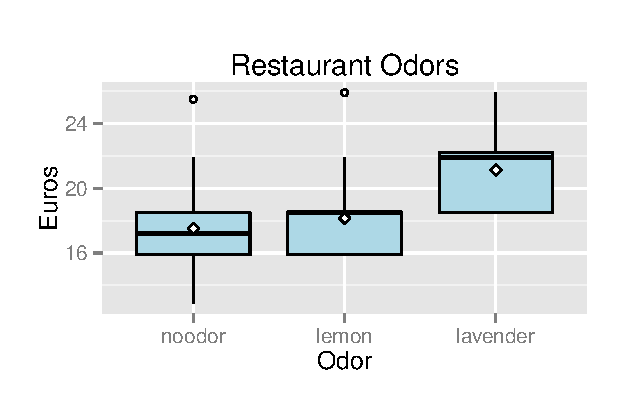
\includegraphics{figures/ex44.eps}
          \caption{Exercise 44}
        \end{figure}

        It looks like either odor makes people spend more money but lavender is more effective than lemon.

      \item[50]
        \begin{table}[H]
          \centering
          \begin{tabular}{rl}
            \toprule
            Min.    & 0.1 \\
            1st Qu. & 0.975 \\
            Median  & 3.3 \\
            Mean    & 4.727 \\
            3rd Qu. & 7.2 \\
            Max.    & 19.6 \\
            \bottomrule
          \end{tabular}
        \end{table}

        Since the mean is larger than the median, the distribution is right-skewed.

        US, Canada, and Australia are outliers according to the rule.  This makes sense when you look at the histogram
        or stem plot.

        \begin{figure}[H]
          \centering
          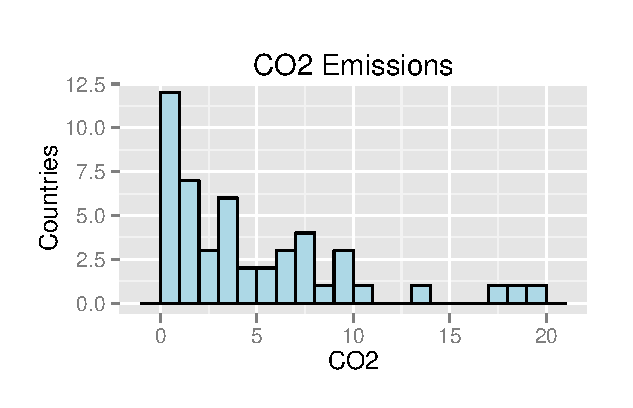
\includegraphics{figures/ex50.eps}
          \caption{Exercise 50}
        \end{figure}
    \end{description}

  \else
    \vspace{11 cm}
    \begin{quote}
      \begin{em}
        Even voting for the right is doing nothing for it. It is only expressing to men feebly your desire that it
        should prevail. 
        % A wise man will not leave the right to the mercy of chance, nor wish it to prevail through the power of the
        % majority. There is but little virtue in the action of masses of men. When the majority shall at length vote for
        % the abolition of slavery, it will be because they are indifferent to slavery, or because there is but little
        % slavery left to be abolished by their vote. 
      \end{em}
    \end{quote}
    \hspace{1 cm} --Henry David Thoreau
  \fi

\end{document}

